\documentclass{article}

\usepackage{arxiv}

\usepackage[utf8]{inputenc} % allow utf-8 input
\usepackage[T1]{fontenc}    % use 8-bit T1 fonts
\usepackage{lmodern}        % https://github.com/rstudio/rticles/issues/343
\usepackage{hyperref}       % hyperlinks
\usepackage{url}            % simple URL typesetting
\usepackage{booktabs}       % professional-quality tables
\usepackage{amsfonts}       % blackboard math symbols
\usepackage{nicefrac}       % compact symbols for 1/2, etc.
\usepackage{microtype}      % microtypography
\usepackage{graphicx}

\title{Functional Data Analysis of EEG Data: Comparing Alcoholics and
Controls}

\author{
  }


% tightlist command for lists without linebreak
\providecommand{\tightlist}{%
  \setlength{\itemsep}{0pt}\setlength{\parskip}{0pt}}



\begin{document}
\maketitle


\begin{abstract}

\end{abstract}


\begin{center}\rule{0.5\linewidth}{0.5pt}\end{center}

\subsection{Background:}\label{background}

Alcoholism can be associated as a catalyst for cognitive decline and
altered brain function, however detecting consistent neural markers is
considered challenging. Electroencephalography (EEG) provides a
non-invasive method to measure brain activity using precise time
measurements whilst offering a non-invasive method to help explore the
presented differences. Many EEG studies tend to rely heavily on average
responses/peak amplitudes which discards imperative information about
how the brain's response changes over time.

\subsection{Aims:}\label{aims}

This study investigates whether differences in EEG signal shape can
distinguish alcoholic from control participants, using a data-driven
approach that captures the full temporal structure of the signals.

\subsection{Methods:}\label{methods}

We applied Functional Data Analysis (FDA) to given EEG signals collected
from alcoholic and control participants who took part in various visual
stimuli related tasks. We represented the EEG signals as smooth
continuous curves to preserve their temporal shape. Functional Principal
Component Analysis (FPCA) to extract key patterns in variation. These
key patterns, otherwise known as components, were utilised during
clustering and classification, testing whether EEG shape alone can
distinguish between the subject identifiers (alcohols or controls).

\subsection{Expected Outcomes:}\label{expected-outcomes}

We expect to find that group differences in EEG signals are most
pronounced during unexpected stimuli conditions, for example the S2
No-Match task. These findings would reflect an altered cognitive
processing in alcoholics. We also anticipate that FPCA components when
used with machine learning classifiers, eg random forests, will offer a
moderate to strong predicative performance in distinguishing group
status based solely on EEG signal shape.

\begin{center}\rule{0.5\linewidth}{0.5pt}\end{center}

\tableofcontents
\newpage

\begin{center}\rule{0.5\linewidth}{0.5pt}\end{center}

\section{Introduction}\label{introduction}

\subsection{Context:}\label{context}

Alcohol use disorder (AUD) has been linked to impairments in cognitive
control, attention, and stimulus processing. Individuals with AUD often
show deficits in tasks requiring cognitive control and flexibility,
these effects from changes are believed to have measurable neural
correlates. EEG provides a non-invasive method of capturing brain
activity with millisecond-level precision and is thus well-suited for
studying cognitive processing in real-time.

\subsection{Why EEG?}\label{why-eeg}

EEG offers several advantages for studying brain function: it is
cost-effective, non-invasive, and highly sensitive to the rapid temporal
dynamics of cognitive processes. This makes it an ideal tool for
comparing brain responses between groups with subtle neurological
differences, such as alcoholics and controls.

\subsection{Stimuli and Sensor
Selection}\label{stimuli-and-sensor-selection}

In this study, participants were exposed to three types of visual
stimuli:

\begin{itemize}
\item
  S1 (Object): A single image,
\item
  S2 Match: Two identical images,
\item
  S2 No-Match: Two different images.
\end{itemize}

These conditions were designed to test how the brain responds to
repeated versus unexpected visual inputs.

EEG signals were recorded using 64 electrodes across the scalp, but our
analysis focused on two frontal sites: FP1 and FP2. These electrodes
were chosen because frontal regions are closely associated with
cognitive function, attention, and decision making, all of which are
areas known to be affected by alcohol use. Focusing on FP1 and FP2 also
helped reduce data complexity while still capturing meaningful
differences in brain response.

\subsection{What Has Been Done Before: EEG Studies in Alcoholism
Research}\label{what-has-been-done-before-eeg-studies-in-alcoholism-research}

There is a substantial amount of EEG research that have investigated
cognitive dysfunction associated with alcohol use disorder. Many of
these studies focus on event-related potentials (ERPs), which are
averaged EEG responses that are time-locked to stimulus presentation.
One commonly studied ERP is the `P300 component', which typically
appears 300 milliseconds after a rare/unexpected stimulus and reflects
attention and stimulus evaluation processes.

From previous studies there is a consistent patterns of participants
with AUD showing a lower P300 amplitude, this would indicate weaker
cognitive processing. A study example `Polish et al (1994)' reported
that the P300 responses for alcoholics were reported to be smaller
during oddball tasks which would allude to reduced attention. Similarly
`Porjesz and Begleiter (2003)' reviewed ERP and suggested that a lower
P300 may even reflect a genetic risk factor for alcoholism.

\subsection{Other studies (e.g.~Kamarajan et
al.~2006)}\label{other-studies-e.g.-kamarajan-et-al.-2006}

have used the basic features of EEG signals by utilising findings such
as average voltage, peak amplitudes and/or response time to compare
alcoholics and non-alcoholics. These studies tend to focus on particular
parts of the EEG signal, making the data easier to work with but in
return losing a lot of time-related details. (Rangaswamy et al, 2007)

\subsection{Limitations of Prior Work}\label{limitations-of-prior-work}

Traditional EEG analysis techniques reduce complex, time-varying signals
to single summary statistics. This approach risks oversimplifying the
data---for instance, two signals might have the same peak amplitude but
very different trajectories before and after the peak. Moreover, these
methods often rely on assumptions like normality that may not hold.

Very few studies have retained the full shape of EEG signals in their
analyses, and even fewer have applied this approach in the context of
alcohol-related research.

\subsection{Gap in the Literature:}\label{gap-in-the-literature}

As previously stated, the aforementioned studies relied heavily on
single-point summaries, indicating the EEGs overall shape, how it rises
and falls and fluctuates over time is being ignored. Basing it off
factors such as peak amplitude or means can be seen as a major
limitation. For example two participants may have the same peak value
but show completely different signal patterns leading up and following
this peak value. Traditional methods miss these key differences which
left a gap for a study that utilises these time-based differences.

\subsection{Our Approach and
Motivation:}\label{our-approach-and-motivation}

In these study, we aim to move beyond summary statistics and keep the
entire time-based structure on the EEG signals we decided to focus on.
We utilised Functional Data Analysis, to ensure each EEG trial was
treated as a continuous curve rather than isolated points. FPCA allowed
us to breakdown the EEG data into a set of shape-based components that
kept the key patterns and differences. These components were later used
to explore clustering too group similar patterns together and
classification to predict a subject identifier (control or alcoholic).

\subsection{Research Aims and
Questions:}\label{research-aims-and-questions}

This project was guided by the following research questions:

\begin{enumerate}
\def\labelenumi{\arabic{enumi}.}
\item
  Do EEG patterns differ between alcoholics and controls?
\item
  How do different visual stimuli (S1 -- Object, S2 -- Match, and S2 --
  No-Match) affect EEG signals?
\item
  Can EEG curve shapes be used to group participants using clustering
  methods?
\item
  Can we predict group membership (alcoholic or control) from EEG data
  using classification models?
\end{enumerate}

\begin{center}\rule{0.5\linewidth}{0.5pt}\end{center}

\section{Methods}\label{methods-1}

\subsection{Data Description}\label{data-description}

The dataset used throughout our studies was obtained from UCI Machine
Learning Repository which was hosted on Kaggle:
\url{https://www.kaggle.com/datasets/nnair25/Alcoholics}.

This dataset contains 16 participants divided into two groups 8
alcoholics and 8 control subjects. Each participant undertook various
trials where they were exposed to various visual stimuli while their
brain activity was recorded by 64 electrodes. These electrodes were
positioned on the scalp following the International 10 -- 20 System.

EEG signals were sampled at 256 Hz, which provides a datapoint at
approximately every 3.9 milliseconds. The trials lasted one second and
contained 265 time points per trial. The given data included multiple
trials per multiple subject, however, for our study we focussed on the
first trial from each participant for each stimuli to ensure consistency

\subsubsection{Visual Stimuli
Conditions:}\label{visual-stimuli-conditions}

Each participant was shown images from Snodgrass \& Vanderwart
standardised picture set (1980) under three different conditions.

\begin{itemize}
\item
  S1 Object: A single image presented from the picture set
\item
  S2 Match: Two identical images presented sequentially from the picture
  set
\item
  S2 No-Match: Two different images presented sequentially from the
  picture set
\end{itemize}

The aim for these conditions was to test how the brain responds to
visual repetition versus unexpected change. The S2 No-Match condition
introduces an unexpected mismatch requiring increased processing which
is expected to evoke a stronger cognitive response.

\subsubsection{Electrode Selection:}\label{electrode-selection}

Although data was recorded from all 64 electrode sensors, our analysis
focused on two frontal electrodes in particular FP1 \& FP2
(\url{https://commons.wikimedia.org/wiki/File:EEG_10-10_system_with_additional_information.svg})

\begin{figure}[H]
\centering
\includegraphics[width=0.4\textwidth]{images/brain_diagram.png}
\caption{EEG Electrode Layout and Associated Brain Regions.}
\end{figure}

These electrodes were selected for our study as frontal brain regions
are known the play a key role in attention, inhibition and cognitive
function, all of which are often impaired with over consumption of
alcohol or AUD. Focussing on these two frontal sensors allowed us to
capture meaningful insight into the differences in brain function based
off these domains, while reducing computational complexity. These
electrodes are often focussed on in previous EEG \& ERP studies
investigating alcohol-related processing, making them theoretically and
practically justified as focal points for our analysis.

\begin{center}\rule{0.5\linewidth}{0.5pt}\end{center}

\subsection{Pre-processing \& Smoothing}\label{pre-processing-smoothing}

Before Analysis, the raw EEG signals underwent pre-processing to reduce
noise and prepare for curve-based modelling. Originally, each trial
recorded 256 discrete time points, subsequently, these points were
smoothed into a continuous function using B-spline basis functions. This
approach allowed us to treat these EEG signals as curves and extract
meaningful patterns across a given time period. This smoothing process
was a crucial step to prepare the data for later Functional Principle
Component Analysis (FPCA), which relies on capturing overall shape and
investigating key components.

\subsubsection{B-Spline Smoothing}\label{b-spline-smoothing}

Initially, we applied B-spline basis functions to model the EEG signals
as continuous functions. The smoothing parameter was chosen using
cross-validation to strike a balance between overfitting and
underfitting, ensuring enough flexibility to capture the underlying
signal while avoiding noise. This process was essential for enabling
FPCA later in the pipeline, which requires smooth, comparable functions.

\subsubsection{Fourier Smoothing}\label{fourier-smoothing}

Although B-splines provided reasonable approximations, we later adopted
Fourier basis functions to better reflect the oscillatory and periodic
nature of EEG signals. Fourier basis functions, built from sine and
cosine waves, are particularly well suited for EEG data, which often
display rhythmic patterns over time.

\subsubsection{Comparison of Basis
Functions}\label{comparison-of-basis-functions}

Visual inspection (see Figure 2) showed both B-spline and Fourier
smoothing yielded similar overall fits. However, Fourier smoothing
produced more globally smooth and consistent wave-like curves, which may
have contributed to improved model performance in prediction tasks. As a
result, Fourier smoothing was used in our later modelling and FPCA
stages.

\begin{figure}[H]
\centering
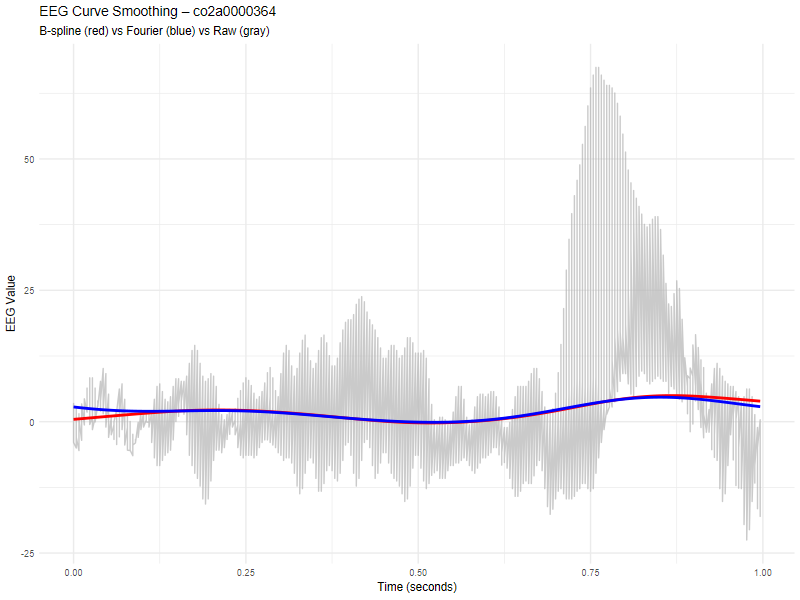
\includegraphics[width=0.4\textwidth]{images/eeg_curve.png}
\caption{EEG Curve Smoothing.}
\end{figure}

\subsubsection{Smoothing Comparison: B-spline vs
Fourier}\label{smoothing-comparison-b-spline-vs-fourier}

Why add: Demonstrates why Fourier was chosen for final FPCA. Visual
evidence supports methodology.

Where to add: In Section 2.2 (Pre-processing \& Smoothing) or Section
2.4 (FDA).

What to show: Same EEG curve smoothed with both methods side-by-side.

Optional but helpful. Especially if you want to justify model decisions
clearly.

\begin{center}\rule{0.5\linewidth}{0.5pt}\end{center}

\subsection{Permutation Testing}\label{permutation-testing}

A central aim throughout this study was to determine whether
statistically significant differences exist between the control and
alcoholic participant's EEG signals. Due to EEG data typically being
high dimensional, non-normally distributed and noisy, traditional
parametric statistical tests such as ANOVA \& t-test are not appropriate
in this context. To address this, we applied a permutation test. A
permutation test is a non-parametric method that makes no assumptions
about the underlying distribution of the data, which is far more
reliable for this context.

\subsubsection{Rationale for Permutation
Test:}\label{rationale-for-permutation-test}

Throughout this study we utilised this test type to assess whether the
observed differences between the subject identifier's (alcoholic's
vs.~control's) average EEG curves were greater than what would be
expected to occur by chance. This step is crucial for evaluating our
first research question (Research Question 1) which asked whether EEG
patterns differ between subject identifier groups.

\subsubsection{How it works:}\label{how-it-works}

We initially focused on the FP1 electrode and ran the test separately
for each of the three stimulus conditions (S1 obj, S2 Match and S2
No-Match) for condition group the steps are as follows: 1. Compute the
Observed Test Statistic

Calculate the pointwise differences in mean EEG curves between the two
subject identifiers (alcoholic and controls). This gives a curve
representing the observed group difference over time.

\begin{enumerate}
\def\labelenumi{\arabic{enumi}.}
\setcounter{enumi}{1}
\tightlist
\item
  Generate a null distribution
\end{enumerate}

Randomly shuffle the group labels (alcoholic/control) 1000 times, and
with each shuffle recalculate the group difference to create a
distribution of test statistics under the null hypothesis (in this case
no group effect).

3.Calculate a p-value

We compared the observed test statistic to the null distribution. The
p-value was defined as the proportion of permuted test statistics that
were greater than or equal to the observed value. A low p-value (p
\textless{} 0.05) indicates that the observed group difference is
unlikely to have occurred by chance.

\subsubsection{Why This Approach is
Appropriate:}\label{why-this-approach-is-appropriate}

Permutation testing aligns well with the nature of EEG data. It not only
avoids assumptions of normality but also respects the time-dependent
structure of EEG curves, by retaining the full functional form of the
EEG curves. It provides a distribution-free method for inference,
increasing confidence in results derived from a modest sample size, such
as ours (n = 16).

\begin{center}\rule{0.5\linewidth}{0.5pt}\end{center}

\subsection{Functional Data Analysis
(FDA)}\label{functional-data-analysis-fda}

Following the findings from permutation tests, which revealed meaningful
group-level differences in EEG signal shape, particularly under the S2
No-Match condition. FDA provided a powerful way to preserve the temporal
structure of the EEG signals and move beyond traditional methods that
rely on single-point summaries like peak amplitude or mean response.

\subsubsection{Why Functional Data
Analysis?}\label{why-functional-data-analysis}

Traditional EEG analysis methods often reduce signals to summary
statistics such as peak amplitude or means. While these are informative,
they discard a lot of the temporal information of the curve. They ignore
the rich, time-varying structure of the data, masking important
differences between groups. FDA retains the full shape of the curve,
capturing how the signal rises, falls, and fluctuates over all time
points.

FDA allows us to represent each trial as a smooth function. This is
important for identifying dominant patterns of variability over time and
reduce noise through curve smoothing. FDA also gives a component for
each curve which represents the key patterns of variation which assists
in the Functional Principal Component Analysis.

\subsubsection{Smoothing and Basis
Functions:}\label{smoothing-and-basis-functions}

Each raw EEG signal was recorded at 256 discrete time points over a
one-second trial. To convert these into functional smoothed curves, we
explored two different types of basis functions.

\subsubsection{B-Spline Basis
Functions:}\label{b-spline-basis-functions}

Localised polynomial functions that are flexible and perform well when
signals vary rapidly in certain time windows. These were initially used
with cubic splines and tuning via cross-validation.

\subsubsection{Fourier Basis Functions:}\label{fourier-basis-functions}

Built from sine and cosine waves, these are ideal for modelling
periodic, rhythmic data, such as EEG signals. Fourier basis functions
provide a more global and concise representation, particularly when the
signal exhibits smooth, wave-like patterns.

\subsubsection{Comparison and Final
Choice:}\label{comparison-and-final-choice}

Initially, we focused on cubic B-Splines for our analysis using
cross-validation to avoid overfitting. However, upon further research we
discovered Fourier basis functions. We found they offered a more
interpretable and concise representation of the underlying EEG patterns,
with fewer basis functions needed to capture the same signal complexity.

After comparing both approaches, our final smoothing decision was to use
Fourier basis functions with 7 basis elements in our FPCA. We found that
this balanced model simplicity and curve integrity. Visual inspection of
smoothed curves showed that Fourier-based representations offered more
consistent reconstructions across participants and stimulus conditions.
These comparisons supported the use of Fourier basis functions in the
next stage of analysis.

\subsubsection{Preparing for Functional Principal Component
Analysis}\label{preparing-for-functional-principal-component-analysis}

With each EEG signal now expressed as a smooth functional component, we
can apply FPCA. This will allow us to extract key shape-based components
from the data, revealing dominant modes of variability across subjects.
This step marked the transition from signal representation to functional
modelling, forming the backbone of the next analytical stages.

\begin{center}\rule{0.5\linewidth}{0.5pt}\end{center}

\subsection{Functional Principal Component Analysis
(FPCA)}\label{functional-principal-component-analysis-fpca}

After smoothing each EEG signal into a continuous functional curve using
basis functions, we applied Functional Principal Component Analysis
(FPCA) to identify dominant patterns/components of variation across the
subjects.

FPCA is a foundational tool in FDA. Its approach is to break each
subject's EEG curve down into a mean function alongside a weighted sum
of principal components (otherwise known as eigenfunctions or modes of
variation).

Mathematically, each EEG curve can be expressed as a sum of shape-based
components:

\[
X_i(t) = \mu(t) + \sum_{k=1}^{K} \xi_{ik} \phi_k(t)
\]

where is the mean curve, are the principal components (eigenfunctions),
and are the scores for subject i on component .

Each principal component helps capture a distinct shape feature in the
data, such as changes in amplitude, timing, and curvature. The scores
assigned to each component for a given subject suggest how strongly that
subject's signal expresses that key feature.

\subsubsection{How FPCA was used:}\label{how-fpca-was-used}

FPCA was applied separately to FP1 and FP2 electrodes, for each trials
smoothed EEG signal. We initially extracted 10 components per electrode,
but retained the first 6 for further analysis, as these collectively
explained the vast majority of variance. Specifically, the first three
components typically covered over 90\% of the total variance:

\begin{itemize}
\item
  PC1 typically captured overall amplitude differences.
\item
  PC2 represented latency shifts (timing of peaks).
\item
  PC3 captured more subtle, localised shape variations.
\end{itemize}

Each EEG signal was thus represented by a vector of FPCA scores (e.g PC1
-- PC6), this summarised their EEG signal shape in a low-dimensional but
meaningful, informative way. These scores were subsequently used as
input features for clustering and classification models. These FPCA
scores formed the core feature set for subsequent clustering and
classification modelling, allowing us to analyse EEG shape across
participants without discarding critical temporal structure.

\begin{enumerate}
\def\labelenumi{\arabic{enumi}.}
\setcounter{enumi}{2}
\tightlist
\item
  FPCA Component Visuals Why add: Your presentation shows these
  graphically --- they help the reader see what each PC is capturing
  (amplitude, timing shifts, etc.).
\end{enumerate}

Where to add: In Section 2.5 (FPCA) or in Results -- RQ2.

What to show: First 2--3 eigenfunctions for FP1 and/or FP2, optionally
alongside the mean function (t).

Nice-to-have. Makes the abstract concepts concrete.

\begin{center}\rule{0.5\linewidth}{0.5pt}\end{center}

\subsection{Functional Principal Component Analysis
(FPCA)}\label{functional-principal-component-analysis-fpca-1}

After smoothing each EEG signal into a continuous functional curve using
basis functions, we applied Functional Principal Component Analysis
(FPCA) to identify dominant patterns/components of variation across the
subjects.

FPCA is a foundational tool in FDA. Its approach is to break each
subject's EEG curve down into a mean function alongside a weighted sum
of principal components (otherwise known as eigenfunctions or modes of
variation). Each principal component helps capture a distinct shape
feature in the data, such as changes in amplitude, timing, and
curvature. The scores assigned to each component for a given subject
suggest how strongly that subject's signal expresses that key feature.

\subsubsection{How FPCA was used:}\label{how-fpca-was-used-1}

FPCA was applied separately to the FP1 and FP2 electrodes, for each
trial's smoothed EEG signal. We initially extracted 10 components per
electrode, but retained the first 6 for further analysis, as these
collectively explained the vast majority of variance. Specifically, the
first three components typically covered over 90\% of the total
variance:

\begin{itemize}
\item
  PC1 typically captured overall amplitude differences.
\item
  PC2 represented latency shifts (timing of peaks).
\item
  PC3 captured more subtle, localised shape variations.
\end{itemize}

Each EEG signal was thus represented by a vector of FPCA scores (e.g.,
PC1--PC6). This summarised their EEG signal shape in a low-dimensional
but meaningful and informative way. These scores were subsequently used
as input features for clustering and classification models.

These FPCA scores formed the core feature set for subsequent clustering
and classification modelling, allowing us to analyse EEG shape across
participants without discarding critical temporal structure.

Mathematically, each EEG curve can be expressed as a sum of shape-based
components:

Picture

where {[}Equation{]} is the mean curve, {[}Equation{]}{[}Equation{]}are
the principal components (eigenfunctions), and {[}Equation{]} are the
scores for subject i on component {[}Equation{]}.

\begin{center}\rule{0.5\linewidth}{0.5pt}\end{center}

\subsection{Clustering}\label{clustering}

Following the extraction of key shape-based features from FPCA, we
employed unsupervised clustering to explore whether EEG signal shapes
alone could reveal meaningful groupings among participant trials,
particularly with respect to alcoholism status and stimulus type.

\subsubsection{Clustering Algorithm:
K-Means}\label{clustering-algorithm-k-means}

We selected K-means clustering as our primary algorithm due to its
simplicity, interpretability, and effectiveness in identifying compact,
spherical clusters in multidimensional space. K-means partitions data
into k groups by minimising the within-cluster sum of squares, assigning
each observation to the nearest cluster centroid.

While more complex algorithms could also be applied such as hierarchical
clustering, we found K-means provided a conceptually clear and
computationally efficient approach to explore the latent structure in
the FPCA score space.

\subsubsection{Input Features}\label{input-features}

The clustering was performed on the combined FPCA score matrix, which
included the first six principal components from both FP1 and FP2
electrodes. These components represented the most important modes of
variation in EEG signal shape and provided a low-dimensional summary of
each participant's response.

\begin{itemize}
\item
  Each row in the input matrix corresponded to a participant-trial.
\item
  Each column represented a principal component score, capturing
  variation in signal shape (e.g.~amplitude, latency, waveform pattern).
\end{itemize}

We retained only those components explaining substantial variance,
ensuring the clustering was driven by meaningful differences.

Combining FP1 and FP2 information allowed us to represent frontal brain
activity comprehensively while preserving electrode-specific
contributions.

\subsubsection{Determining the Number of
Clusters}\label{determining-the-number-of-clusters}

To select the optimal number of clusters (k), we explored:

\begin{itemize}
\item
  Elbow plots: plotting total within-cluster variance across a range of
  k values to identify diminishing returns.
\item
  Silhouette analysis: measuring how similar each observation is to its
  own cluster versus others.
\end{itemize}

These diagnostics, along with theoretical considerations of
task/stimulus types and expected heterogeneity, led us to focus on k = 3
as a meaningful partition of the data.

\subsubsection{Visualisation and
Interpretation}\label{visualisation-and-interpretation}

Once each trial was assigned to a cluster, we performed the following
analyses to interpret the clustering structure:

\begin{itemize}
\item
  Visualise clusters in principal component space.
\item
  Overlay clusters on raw EEG curves, coloured by membership, to examine
  whether clusters represented distinct waveform shapes.
\item
  Compare cluster compositions with known group labels (alcoholic vs
  control) and stimuli, to evaluate whether natural groupings aligned
  with meaningful clinical or experimental categories.
\end{itemize}

These visualisations allowed us to assess whether clusters reflected
meaningful differences in EEG shape and whether they aligned with group
status or stimulus condition, highlighting the potential of EEG curve
features to reveal underlying structure without supervision.

\begin{center}\rule{0.5\linewidth}{0.5pt}\end{center}

\subsection{Classification Modelling}\label{classification-modelling}

Having established that EEG signal shape differs between alcoholics and
controls through permutation testing, and that unsupervised clustering
reveals latent structure in the data, we next explored whether these
differences could be used to predict group membership. Specifically, we
tested whether a participant's alcoholism status could be predicted
based on FPCA-derived features.

To achieve this, we trained and compared multiple supervised
classification models using the principal component scores as input
features.

\subsubsection{Feature Set: FPCA Scores}\label{feature-set-fpca-scores}

The input for all models was a feature matrix consisting of the first
six principal component scores extracted via FPCA from FP1 and FP2
electrodes. These scores compactly represent the shape of each EEG
curve, summarising its most important temporal features.

Each row represented one trial, and the outcome variable was binary:

\begin{itemize}
\item
  1 = Alcoholic
\item
  0 = Control
\end{itemize}

To prevent overfitting and allow generalisation, we used a train-test
split (70/30), and evaluated model performance on the unseen test set.

\subsubsection{Lasso Logistic
Regression}\label{lasso-logistic-regression}

Rationale: Lasso (Least Absolute Shrinkage and Selection Operator) is a
penalised regression method that performs variable selection and
regularisation. It is particularly well-suited to high-dimensional data
like FPCA scores, where only a subset of features may be relevant.

Implementation: We applied Lasso logistic regression using 10-fold
cross-validation to select the regularisation parameter that minimised
classification error.

Advantages:

\begin{itemize}
\item
  Automatically reduces less relevant FPCA components.
\item
  Produces interpretable models by shrinking coefficients to zero.
\end{itemize}

\subsubsection{Random Forest}\label{random-forest}

Rationale: Random Forest is a tree-based ensemble method that aggregates
predictions from multiple decision trees, reducing variance and
improving accuracy. It is non-parametric and can capture nonlinear
interactions between predictors.

Implementation: We trained a Random Forest classifier using default
parameters, tuning the number of trees and variables per split (mtry)
based on out-of-bag error.

Advantages:

\begin{itemize}
\item
  Robust to outliers and overfitting.
\item
  Captures complex interactions between components.
\item
  Provides variable importance metrics, indicating which PCs contributed
  most to prediction.
\end{itemize}

\subsubsection{Multinomial Logistic
Regression}\label{multinomial-logistic-regression}

Rationale: Although our primary classification task is binary (alcoholic
vs.~control), we also considered stimulus condition (S1, S2 Match, S2
No-Match) as an outcome, allowing the use of multinomial logistic
regression for exploratory purposes.

Implementation: We fitted a multinomial logit model using FPCA scores as
predictors, and evaluated its performance on correctly classifying
trials by stimulus condition.

Advantages:

\begin{itemize}
\item
  Allows extension to multiclass problems.
\item
  Provides a baseline comparison to more complex methods.
\end{itemize}

\subsubsection{Model Evaluation}\label{model-evaluation}

To investigate the performance of our classification models, we assessed
the following standard evaluation metrics:

\begin{itemize}
\item
  Accuracy: The proportion of correctly predicted labels out of the
  number of predictions made. Used to give an overall sense of model
  performance.
\item
  Sensitivity (True Positive Rate): The proportion of alcoholic
  participants correctly identified as alcoholics. This can be important
  for scenarios where filing to detect alcoholism is more detrimental
  than a false alarm.
\item
  Specificity (True Negative Rate): The proportion of controls who were
  correctly classified as non-alcoholics. High specificity indicates the
  model is not producing false positives by identifying healthy
  individuals as alcoholic. We ensured to utilise confusion matrices to
  visualise the breakdown if true/false positives and negatives for each
  of the models.
\end{itemize}

Picture This allowed us to interpret model performance in a more
detailed way opposed to a single accuracy score. These metrics were
calculated for each of the classifiers e.g.~Random Forest, Lasso and
Multinomial Logistic Regression, as well as each basis function (Fourier
\& B-Spline). This gave us the opportunity to efficiently compare their
effectiveness in predicting group status from FPCA scores.

\begin{figure}[H]
\centering
\includegraphics[width=0.4\textwidth]{images/confusion_matrix.png}
\caption{Confusion Matrix}
\end{figure}

\begin{center}\rule{0.5\linewidth}{0.5pt}\end{center}

\section{Results}\label{results}

\subsection{RQ1: Do EEG patterns differ between alcoholics and
controls.}\label{rq1-do-eeg-patterns-differ-between-alcoholics-and-controls.}

This research question involved testing group-level differences,
particularly in shape.

To address RQ1, we plotted the mean EEG curves for both groups across
each visual stimuli.

As seen in Fig 4, the S2 No-Match condition shows the greatest
divergence in EEG curve shape between groups. We began by plotting the
mean EEG responses for alcoholics and controls across all stimulus
types, which motivated a subsequent permutation test to assess
statistical significance.

\begin{figure}[H]
\centering
\includegraphics[width=0.4\textwidth]{images/mean_eeg.png}
\caption{Mean EEG Curve}
\end{figure}

The permutation test for the S2 No-Match condition returned a p-value of
0.021, indicating a statistically significant difference between
alcoholics and controls. As shown in Fig 5, the observed test statistic
(red dashed line) lies in the extreme right tail of the null
distribution, meaning such a result is unlikely to occur by chance.

\begin{figure}[H]
\centering
\includegraphics[width=0.4\textwidth]{images/perm_test.png}
\caption{Permutation Test- S2 No-Match}
\end{figure}

In contrast, the S1 and S2 Match conditions did not yield significant
differences (p \textgreater{} 0.05), suggesting more similar neural
responses between groups for simpler or repeated visual stimuli.

These findings support the hypothesis that group-level differences are
most pronounced under cognitively demanding conditions, like when
unexpected stimuli are presented (S2 No-Match).

\subsection{RQ2: How do different visual stimuli affect EEG
signals?}\label{rq2-how-do-different-visual-stimuli-affect-eeg-signals}

This question helped us explore how the signal changes based on the
stimuli type given to participants.

To address Research Question 2, we examined how the shape of EEG signals
varied across the three stimulus types --- S1 Object, S2 Match, and S2
No-Match --- which differ in levels of cognitive demand.

\begin{figure}[H]
\centering
\includegraphics[width=0.4\textwidth]{images/scores_condition.png}
\caption{FPCA Scores by Stimulus Condition}
\end{figure}

We began by plotting the average smoothed EEG curves for each condition
across all participants. These curves were generated using B-spline
smoothing, which we used in the earlier stages of the project.

At this point in the analysis, Fourier basis had not yet been applied
--- we adopted Fourier later in the pipeline, particularly during FPCA
and modelling stages.

Figure 7 shows that EEG responses to the S2 No-Match condition exhibited
sharper peaks and greater amplitude, consistent with the increased
cognitive effort required to process unexpected visual changes. This
suggests heightened neural activation when detecting novelty.

\begin{figure}[H]
\centering
\includegraphics[width=0.4\textwidth]{images/smooth_mean_eeg.png}
\caption{Smoothed Mean EEG Curve by Stimulus}
\end{figure}

In contrast, the S2 Match condition showed flatter and more variable
curves, indicating a wider range of brain responses across participants.
This variability may reflect the brain's reduced engagement with
repeated stimuli, leading to more diffuse and inconsistent signal
patterns.

These observations support the idea that stimulus type influences both
the intensity and consistency of EEG responses.

To quantify these shape differences, we next examined FPCA scores by
stimulus type --- plotting boxplots of PC1 and PC2 to capture how key
temporal features varied across S1, S2 Match, and S2 No-Match.

Figure 8 shows FPCA score distributions for the first two principal
components. PC1 scores were higher for S1 Object and S2 No-Match,
reflecting stronger average signal features in these conditions. In
contrast, S2 Match showed a dip in PC1 and a wider spread in PC2,
suggesting that repetition led to less consistent waveform shapes across
subjects.

\begin{figure}[H]
\centering
\includegraphics[width=0.4\textwidth]{images/fpca2.png}
\caption{FPCA Scores by Stimulus}
\end{figure}

Visual inspection of the PC1 distributions suggests a difference between
stimulus types, particularly between S1 and S2 No-Match. Future work
could formally test this using a Kruskal-Wallis test or similar
non-parametric method.

\subsection{RQ3: Can EEG Curves Shape Be Used To Group Participants
Using
Clustering?}\label{rq3-can-eeg-curves-shape-be-used-to-group-participants-using-clustering}

Our aim for this question was to explore whether the shape of EEG
signals alone could naturally group participants in a meaningful way,
using subject identifiers and the matching conditions.

After extracting the aforementioned FPCA scores, clustering was applied
to see if the brain signal shapes alone could uncover natural groupings.
This allowed us to explore whether similar EEG patterns emerge across
all participants and identify whether clusters relate to matching
condition (alcoholic/control) or subject identifier (stimulus type).

We visualised the k-mean results utilising scatter lots of the first two
principle components (PC1 \& PC2). Each point representing a
particioant-trial and coloured by assigned cluster. This allowed us to
understand how similar EEG shapes grouped together based on their
component scores.

The cluster-specific stimulus composition mirrors the increasing
cognitive demand across stimuli. This reinforces the idea that FPCA
captures differences in EEG shape and timing that align with the
psychological nature of the task (e.g., novelty or repetition).

\begin{figure}[H]
\centering
\includegraphics[width=0.4\textwidth]{images/image.png}
\caption{Cluster Comparison by FPCA Score}
\end{figure}

Next we looked at what these clusters contained, uncovering whether they
were mostly alcoholics or controls.

While not perfectly separated, the group composition across clusters
shows that unsupervised clustering based on EEG shape features captures
meaningful group-level differences. This supports the potential of FPCA
features in identifying cognitive or neurological groupings without
needing group labels.

\begin{figure}[H]
\centering
\includegraphics[width=0.4\textwidth]{images/image(1).png}
\caption{Cluster Comparison by Group}
\end{figure}

These patterns suggest that EEG curve shapes alone can uncover
meaningful differences in how participants respond to tasks/stimuli,
despite knowing their group label or not.

What They Show: These are summary plots showing how clusters break down
in terms of categorical variables. They do not show the spatial
distribution of the clusters in the PC1 vs PC2 feature space.

What You'd Need for a PC1 vs PC2 Scatter Plot:

X-axis = PC1 score

Y-axis = PC2 score

Color = Cluster assignment (Optional: Shape or label = stimulus/group)

This kind of plot would visually confirm how distinct clusters are in
the reduced 2D space created by FPCA. - should this plot be under
clustering or research question 3 results

Great question --- the PC1 vs PC2 scatter plot with cluster coloring
should be placed under Research Question 3 (RQ3) results, because:

RQ3 Focus:

``Can EEG Curve Shape Be Used to Group Participants Using Clustering?''

This plot directly addresses that question by showing whether the
extracted features (PC1 \& PC2) naturally form separable groups.

How It Fits in RQ3 Structure:

You already have:

Cluster composition by stimulus (bar plot)

Cluster composition by group (bar plot)

Adding the PC1 vs PC2 scatter:

Visually explains why those bar plot differences exist.

Supports the claim that shape-based FPCA features yield meaningful,
separable clusters.

How to Introduce It in RQ3 Section:

``To visualize how well the FPCA-based clusters separate in feature
space, we plotted participant trials by their scores on the first two
principal components (PC1 and PC2), with colors indicating cluster
assignment.''

Then you can add your interpretation based on cluster separation, e.g.,
tight grouping, overlap, or alignment with stimulus/group labels.

\subsection{RQ 4: Can EEG Signal Shape Predict Alcoholism
Status?}\label{rq-4-can-eeg-signal-shape-predict-alcoholism-status}

PictureWe compared two smoothing bases (B-spline and Fourier) combined
with two classifiers: LASSO and Random Forest (RF). Each was evaluated
using three performance metrics: Accuracy, Sensitivity, and Specificity.
(As seen in Figure 11)

\begin{figure}[H]
\centering
\includegraphics[width=0.4\textwidth]{images/model_comparison.png}
\caption{Model Performance Comparison}
\end{figure}

\begin{center}\rule{0.5\linewidth}{0.5pt}\end{center}

\begin{enumerate}
\def\labelenumi{\arabic{enumi}.}
\setcounter{enumi}{3}
\tightlist
\item
  Accuracy vs Components Plot
\end{enumerate}

Why add: In the PDF you mention tuning components (5--7 components) and
that it affects accuracy.

Where to add: In Section 2.7 (Classification Modelling) or after Figure
11 in RQ4.

What to show: Line chart of accuracy vs number of FPCA components (for
RF or Lasso).

Optional advanced detail. Useful if you're highlighting model
optimization.

Unsure if necessary what do you think?

\subsection{Key Findings:}\label{key-findings}

\begin{itemize}
\item
  Fourier + Random Forest outperformed all others, with the highest
  accuracy (\textasciitilde88\%), sensitivity, and specificity.
\item
  B-spline + RF performed second best but slightly below Fourier in all
  metrics.
\item
  LASSO showed relatively lower performance across both basis types,
  especially under Fourier, suggesting it may underfit this type of
  high-dimensional functional data.
\end{itemize}

\subsubsection{Why Fourier Performs
Better:}\label{why-fourier-performs-better}

Fourier smoothing better preserves wave-like oscillatory structure in
EEG signals.

This likely improves feature representation, enabling Random Forest to
more effectively distinguish between alcoholic and control subjects.

\subsubsection{Takeaway:}\label{takeaway}

Using Fourier basis significantly improved predictive performance,
especially with ensemble methods like Random Forest.

\subsection{Confusion Matrix
Interpretation}\label{confusion-matrix-interpretation}

We visualised confusion matrices for both models (LASSO and Random
Forest) using heatmaps. These show how many alcoholic/control
participants were correctly or incorrectly classified.

\subsubsection{LASSO:}\label{lasso}

\begin{itemize}
\item
  Tended to misclassify alcoholics as controls more frequently.
\item
  Shows less separation power between groups.
\end{itemize}

\subsubsection{Random Forest:}\label{random-forest-1}

\begin{itemize}
\item
  Achieved higher counts along the diagonal (true positives and true
  negatives).
\item
  More balanced sensitivity and specificity, indicating better
  generalisation.
\end{itemize}

\subsubsection{Insight:}\label{insight}

Random Forest not only achieved higher accuracy but also avoided group
imbalance. It was more consistent across both alcoholic and control
predictions.

\subsection{Final Graphical
Interpretation}\label{final-graphical-interpretation}

The graphical outputs presented throughout this analysis demonstrate
that EEG signals, when treated as functional data, yield valuable
insight into cognitive processes and group differences. The mean EEG
curves revealed that the S2 No-Match condition produced the strongest,
most defined responses, consistent with the increased cognitive effort
associated with detecting unexpected stimuli.

This observation was statistically validated via permutation testing,
which identified significant differences between alcoholic and control
groups, particularly under the S2 No-Match condition. The FPCA boxplots
further illustrated how key components (PC1 and PC2) varied
systematically with stimulus type, with PC1 capturing amplitude-related
differences and PC2 reflecting variability in temporal signal structure.

Clustering analysis on FPCA scores uncovered coherent structure in the
data: certain clusters were more likely to contain alcoholics or
controls, and others were dominated by specific stimulus conditions.
This suggests that signal shape alone, even without group labels
captures meaningful variation in participant responses.

Lastly, predictive modelling using Lasso and Random Forests confirmed
that these FPCA-derived scores are informative features, achieving
strong classification performance. Notably, models using the Fourier
basis consistently outperformed those using B-splines, likely due to
their ability to better preserve oscillatory EEG structure.

Collectively, the graphical analyses highlight the power of FDA to
extract interpretable, discriminative features from high-dimensional EEG
data, enabling both statistical inference and predictive modelling in a
cognitively meaningful way.

\begin{center}\rule{0.5\linewidth}{0.5pt}\end{center}

\section{Discussion}\label{discussion}

This study set out to investigate whether EEG signal shape could
distinguish between alcoholic and control participants using Functional
Data Analysis (FDA). By treating each EEG signal as a continuous
function and applying Functional Principal Component Analysis (FPCA), we
uncovered meaningful shape-based differences, particularly under
cognitively demanding stimuli. Our results are discussed below in
relation to each research question.

\subsection{RQ1: Do EEG patterns differ between alcoholics and
controls?}\label{rq1-do-eeg-patterns-differ-between-alcoholics-and-controls}

We found significant group-level differences in EEG responses,
particularly under the S2 No-Match condition. The permutation test
confirmed that the divergence in curve shape between alcoholic and
control participants was unlikely to occur by chance (p = 0.021). This
finding suggests that alcoholics exhibit altered neural processing when
faced with unexpected stimuli, consistent with theories of impaired
cognitive flexibility in AUD.

This result aligns with previous ERP literature, particularly studies on
the P300 component. Prior work has shown that alcoholics often display
reduced P300 amplitudes in oddball tasks, indicating attenuated
attentional engagement and stimulus evaluation (Polich et al., 1994;
Porjesz \& Begleiter, 2003). Our functional approach complements and
extends this literature by retaining the full shape of the EEG waveform
rather than focusing on a single latency or peak.

\subsection{RQ2: How do different visual stimuli affect EEG
signals?}\label{rq2-how-do-different-visual-stimuli-affect-eeg-signals-1}

Our results demonstrated that EEG responses varied systematically across
stimulus types. The S2 No-Match condition, designed to introduce
cognitive conflict, elicited the strongest, most structured responses,
while S2 Match (a repetition) generated flatter and more variable EEG
signals. This is consistent with the expected hierarchy of cognitive
demand: repetition (S2 Match) evokes less engagement, while novelty (S2
No-Match) requires heightened processing.

The boxplots of FPCA scores by stimulus type revealed that PC1
(associated with amplitude) was highest for S2 No-Match, while PC2
(timing/variability) was most dispersed for S2 Match. These differences
highlight how shape-based components of the EEG curve change under
different cognitive loads.

\subsection{RQ3: Can EEG shape be used to group
participants?}\label{rq3-can-eeg-shape-be-used-to-group-participants}

Unsupervised clustering on FPCA scores produced meaningful groupings.
Some clusters were enriched for alcoholics or controls, while others
appeared linked to specific stimulus conditions. This suggests that EEG
shape alone, without knowing participant labels, contains enough
information to reveal latent structure related to cognitive traits or
neurological status. These findings support the value of FPCA scores as
compact, interpretable summaries of brain activity.

\subsection{RQ4: Can we predict alcoholism status from EEG
data?}\label{rq4-can-we-predict-alcoholism-status-from-eeg-data}

Yes. Our classification models using FPCA scores from FP1 and FP2
achieved high accuracy, particularly when using Fourier smoothing and
Random Forests (accuracy \textasciitilde{} 85\%). This suggests that
time-domain signal shape, captured through FDA, is a strong predictive
feature for group classification. The superior performance of Fourier
over B-spline likely reflects its ability to capture the rhythmic,
oscillatory nature of EEG.

This approach goes beyond traditional ERP measures by using a richer
summary of the signal and retaining information across the full-time
window. It shows promise for EEG-based screening tools or cognitive
profiling in clinical contexts.

\begin{center}\rule{0.5\linewidth}{0.5pt}\end{center}

\section{Limitations and Future Work}\label{limitations-and-future-work}

\subsection{Limitations}\label{limitations}

\begin{itemize}
\item
  Sample Size: Our dataset included only 16 participants (8 per group),
  limiting statistical power and generalisability. While FDA methods are
  robust for small n, larger datasets would allow for more stable model
  estimation and validation.
\item
  Trial Restriction: We focused on a single trial per stimulus per
  participant to ensure consistency. However, this may omit important
  intra-individual variability.
\item
  Sensor Selection: Although we focused on FP1 and FP2 for theoretical
  and practical reasons, other electrodes (e.g., parietal or occipital
  regions) may capture complementary information, especially for ERP
  components like P300.
\item
  Simplified Modelling: Our modelling used only FPCA scores from frontal
  sites and relatively standard classifiers. More complex architectures
  or incorporating additional features may yield better performance.
\end{itemize}

\subsection{Future Directions}\label{future-directions}

\begin{itemize}
\item
  Multi-trial Functional Modelling: Incorporate repeated measures using
  functional mixed-effects models to account for within-subject
  variation.
\item
  Expand Sensor Coverage: Explore full-scalp FPCA to detect spatial
  patterns in addition to temporal ones.
\item
  Temporal Localisation: Combine FPCA with time-frequency decomposition
  to detect when during the trial group differences emerge.
\item
  Real-time Prediction: Investigate the use of FPCA in online EEG
  decoding and early detection of cognitive impairment.
\item
  Broader Populations: Apply this framework to other populations
  (adolescents, older adults, or clinical cohorts) to test robustness
  and generalisability.
\end{itemize}

\begin{center}\rule{0.5\linewidth}{0.5pt}\end{center}

\section{Conclusion}\label{conclusion}

This study applied Functional Data Analysis (FDA) to EEG signals in
order to explore group-level differences between alcoholic and control
participants and evaluate whether signal shape could be used for
classification and clustering. By treating EEG data as smooth functional
curves and extracting key shape-based components using Functional
Principal Component Analysis (FPCA), we were able to preserve and
interpret the rich temporal dynamics of neural activity.

\subsection{Key findings:}\label{key-findings-1}

\begin{itemize}
\item
  Significant group differences were detected in EEG shape, particularly
  under the S2 No-Match stimulus condition, where alcoholic participants
  exhibited distinct temporal patterns compared to controls.
\item
  Different stimulus types elicited distinct EEG responses, with S2
  No-Match producing stronger and more consistent signals, likely
  reflecting heightened cognitive processing demands.
\item
  Unsupervised clustering using FPCA scores revealed groupings that
  partially aligned with alcoholism status and stimulus condition,
  suggesting that signal shape carries meaningful structure even without
  labels.
\item
  Predictive models using FPCA scores from FP1 and FP2 electrodes
  achieved strong classification performance, especially when Fourier
  basis functions and Random Forests were used.
\end{itemize}

These findings demonstrate the value of functional representations for
analysing complex, high-dimensional time series data like EEG. FDA
methods not only preserve important curve features but also produce
interpretable summaries that support clustering and classification
tasks. This approach offers a promising direction for identifying neural
markers of cognitive dysfunction and could be extended to other domains
within health data science. Future work should expand this analysis to
larger datasets, multiple trials, and additional electrodes, while
exploring more advanced predictive architectures. Nevertheless, this
study provides an important step toward using functional signal shape to
understand and predict cognitive and neurological status. ---

\bibliographystyle{unsrt}
\bibliography{}


\end{document}
